\section{Characterizing Failures using an Intrinsic Signal}
\label{sec:aout_char}
%To study the faults observed in practice in a structured manner, 
Our hypothesis is that the intermediate analog signal (\aout) from the pyroelectric element captures information that is critical to detect various failures. 
%
We now describe how this intrinsic signal and its underlying physics is useful to characterize failures.

\subsection{\aout signal to detect failures in PIR sensors}
\label{subsec:controlled}
As described in \S~\ref{subsec:working}, there are two output signals from a PIR sensor,~\viz \aout and \cout. 
%
The latter is a discrete signal typically used for detecting obstacle presence and is derived from \aout.
%; we show that the signal characteristics of \aout has several key properties.  
%
To show the utility of \aout, we conducted numerous controlled experiments where we manually injected commonly seen faults ({\bfseries Fig.~\ref{fig:pir_sensor_failure_photographs}}). 

% We manually injected failures as shown in {\bfseries Fig.~\ref{fig:pir_sensor_failure_photographs}} and analyzed their impact by comparing with a co-located working sensor. We use a controlled setup for this purpose which is described below and shown in {\bfseries Fig.~\ref{fig:pir_sensor_controlled}}.

% \newenvironment{myquotation}{\setlength{\leftmargin}{1.5em}\quotation}{\endquotation}
% \begin{myquotation}
% 	\noindent\textit{We show that the output signal \aout contains information about the kind of failure present in the PIR sensor. The information about failures is lost from the final discrete output \cout in the process of converting the analog signal \aout into the discrete form.}
% \end{myquotation}

% % \underline{\textbf{Controlled Setup (Microbenchmarking)}} 

Using the setup from {\S\ref{subsec:quantify}}, we co-located two sensors, \tampered and \working, where we change the \tampered sensor to test different types of failures described in \S\ref{subsec:taxonomy}. While in \S\ref{subsec:quantify}, we focused on \cout to study sensor performance during failure, in this experiment we additionally analyze \aout to get an understanding of the \textit{sensor physics} during failure.
%
%: \ci a tampered sensor (\tampered) containing the failure and \cii a working sensor (\working) such that: \ca the distance between the sensors is closer than the size of the obstacle, \cb the obstacle is moved in a plane such that it comes into the detection region of both sensors simultaneously and \cc the obstacle is larger than the distance between the two sensors, allowing it to be incident on both the sensors simultaneously. Thus, we expect the same output from both \tampered and \working. 
%
% This analysis of tampered sensors to working sensors by effecting specific changes is analogous to microbenchmarking in systems software.
%We note the value of \cout for both \tampered and \working. (1 -- when no obstacle, 0 -- when there is obstacle).

%Recall the analysis of output signals of a PIR sensor in \S\ref{subsubsec:working}.
We note the output signals (\ie \aout and \cout) from \tampered in every failure scenario and compare it with that from \working \emph{to understand the impact of failure on physics of the sensors}. Each experiment described below lasted for 15 minutes, where the obstacle (our palm in this case) was moved into the region of detection once every minute. We plot \aout for both a working sensor and every type of faulty sensor in {\bfseries Figs.~\ref{fig:pir_sensor_controlled_a} --~\ref{fig:pir_sensor_controlled_e}}. The y-axis represents voltage output of \aout and x-axis represents time. % upto 900 seconds. 
For the working sensor \working, we expect a spike in \aout once every 60 seconds denoting motion of the palm. Let us now study the nature of \aout in each fault.

\textbf{Lens dislocation (Class I) faults.} The absence/dislocation of the lens causes imperfect focus of thermal radiation resulting in some residual output at the pyroelectric element even when there is no obstacle present. The impact of a Class I fault on \aout is shown in \textbf{Fig.~\ref{fig:pir_sensor_controlled_a}}. 
We can see that both the tampered and working sensors are still able to detect the obstacle (as shown by the 15 vertical spikes of \aout). However, when the obstacle is not present, we observe that the noise of \aout is much higher with a Class I fault as compared to a working sensor. Thus, it is important to look beyond just \cout signal to identify such failures.

\textbf{Lens deformation (Class II) faults.} Class II faults can potentially lead to missing obstacles at the periphery of the field of view due to deformation or loss of material integrity (\eg puncture). 
%The impact of a Class II fault on \aout and \cout is shown in Fig.~\ref{fig:pir_sensor_controlled_b}.
\textbf{Fig.~\ref{fig:pir_sensor_controlled_b}} shows the \aout for a sensor with a Class II fault. The amplitude of \aout at the times of obstacle detection is lower when compared to a working sensor. This is expected since the damage to lens leads to reduced thermal radiation incident on the pyroelectric subsystem. In general, Class II faults creates blind spots in the lens aperture that can reduce amplitude of the \aout signal. 

% \begin{figure*}
% %\centering
% 	\subfloat[\label{fig:pir_sensor_classII_fault_a}]{%
% 		\includegraphics[width=0.66\columnwidth]{figures/2-PIR-Fault/normal-classII/PIR_evm_experiment_raw_dataCout(Normal)-Aout(Normal)Normal-separate.png}}
% 	\subfloat[\label{fig:pir_sensor_classII_fault_b}]{%
% 		\includegraphics[width=0.66\columnwidth]{figures/2-PIR-Fault/normal-classII/PIR_evm_experiment_raw_dataCout(ClassII-LensPuncture)-Aout(ClassII-LensPuncture)ClassII-LensPuncture-separate.png}}
% 	\subfloat[\label{fig:pir_sensor_classII_fault_c}]{%
% 		\includegraphics[width=0.66\columnwidth]{figures/2-PIR-Fault/normal-classII-deformed/PIR_evm_experiment_raw_dataCout(ClassII-LensDeformed)-Aout(ClassII-LensDeformed)ClassII-LensDeformed-separate.png}}
%     \caption{CLASS II Faults (\ref{fig:pir_sensor_classII_fault_a}) \textbf{Response of a Normal Sensor} (\ref{fig:pir_sensor_classII_fault_b}) \textbf{Class II} faulty sensor with lens puncture
%     (\ref{fig:pir_sensor_classII_fault_c}) \textbf{Class II} faulty sensor with lens deformed
%     -- there is very little perceptible difference either in $A_{out}$ or $C_{out}$ in this case. These failures can thus be very insidious and hard to detect from the time-domain analysis.}
% \label{fig:pir_sensor_classII_fault}
% \end{figure*}

\textbf{Lens hindrance (Class III) faults} are caused due to foreign particles entering the lens that compromise its optical capability, thereby affecting the intensity and angle of radiation incident on the pyroelectric element. 
%
We induce such faults by depositing some dust on the lens.
% and observe the difference in output between the normal and faulty case. A scenario demonstrating the presence of Class III fault is shown in Figure~\ref{fig:pir_sensor_controlled_c}.
\textbf{Fig.~\ref{fig:pir_sensor_controlled_c}} shows that the amplitude of \aout varies at each of the detection points. The variation depended on the amount of dust with respect to the orientation of the obstacle. Though the obstacle was still being detected, we note that with increased dust deposition, the amplitude of \aout can fall below the comparator threshold required to capture the obstacle, resulting in a missed obstacle \ie false negative. 
% \footnote{Ref. Appendix for effect of varying dust deposition on \aout.}

%, an effect similar to what would be observed under a Class IV fault.

% \begin{figure}[t]
% %\centering
% 	\subfloat[\label{fig:pir_sensor_classIII_fault_a}]{%
% 		\includegraphics[width=0.49\columnwidth]{figures/2-PIR-Fault/normal-classIII/PIR_evm_experiment_raw_dataCout(Normal)-Aout(Normal)Normal-separate.png}}
% 	\subfloat[\label{fig:pir_sensor_classIII_fault_b}]{%
% 		\includegraphics[width=0.49\columnwidth]{figures/2-PIR-Fault/normal-classIII/PIR_evm_experiment_raw_dataCout(ClassIII-Dust)-Aout(ClassIII-Dust)ClassIII-Dust-separate.png}}
%     \caption{CLASS III Faults -- (\ref{fig:pir_sensor_classIII_fault_a}) \textbf{Response of a Normal Sensor} (\ref{fig:pir_sensor_classIII_fault_b}) \textbf{Class III} faulty sensor with dust deposition on lens
%     -- there is a considerate reduction in amplitude of $A_{out}$ as compared to the normal sensor though the $C_{out}$ in this case demonstrates the reference obstacle being detected. The amount of reduction is proportional to the amount of dust deposited.}
% \label{fig:pir_sensor_classIII_fault}
% \end{figure}


\textbf{Failure in pyroelectric components (Class IV).} Class IV faults happen when the optical filter on the pyroelectric element comes in contact with contaminants such as oil, mist or other smudge, resulting in potentially missing obstacles. High temperatures can also cause expansion of the optical filter that can also result in failures. 
We induce Class IV faults by spraying some oil on the optical filter. We observe in {\bfseries Fig~\ref{fig:pir_sensor_controlled_d}} that \aout has significantly attenuated spikes at each of the points that correspond to obstacle motion, but the spikes are not high enough to cause \cout to drop LOW. This results in the obstacle to be missed completely. A similar effect is observed when the optical filter is exposed to heat as it affects the temperature variation needed for pyroelectric effect.

%\textbf{Summary (Figure~\ref{fig:pir_sensor_controlled_d})} We note that in the case, there are small spikes of \aout at each of the points in time where there is obstacle motion. However, \cout remains HIGH in all the cases implying that the obstacle is missed resulting in a \textit{complete failure}. Note that the degree of failure depends on the magnitude of contamination and the severity of the deployed environment. 

\textbf{Failure in electronics (Class V) faults.} Class V faults are typically electronic faults such as short or open circuits. They can cause the \aout or \cout values to be `stuck' at certain anomalous value such as HIGH (3.3 V) or LOW (0 V). As a result, these failures can cause the obstacle to be completely missed. This is observed in {\bfseries Fig.~\ref{fig:pir_sensor_controlled_e}}, where \aout is shorted to the power supply, resulting in \cout following \aout and remaining HIGH. Consequently, the \aout waveform here is a flat, horizontal line and lacks oscillations. 
%
%\textbf{Summary:} Based on the above analysis, we see that the output signal \aout contains information about the kind of failure present in the PIR sensor. Further, this information is lost from the final discrete output \cout in the process of converting the analog signal \aout into the discrete form.

\noindent \textbf{Summary:} The core insight here is that \aout can shed light on the physical and electrical operating conditions of a PIR sensor as opposed to the mere boolean occupancy indicated by \cout. Thus, being able to snoop in on \aout can capture the interaction of IR radiation on the different sensor subsystems. 
%We need to talk about why Aout is giving such information so physics would be good to add here.

%\textbf{Summary (Figure~\ref{fig:pir_sensor_controlled_e})} In this case, we see that the \aout is shorted to the power supply and thus results in \cout following \aout and remaining HIGH, resulting in the obstacle (that arrived at the same points in time as shown in Figs~\ref{fig:pir_sensor_controlled_a} --~\ref{fig:pir_sensor_controlled_c}, ~\ref{fig:pir_sensor_controlled_d}) being completely missed.

\subsection{Analysis of \aout during partial failures and gradual degradation} \label{subsec:incremental_dust}In \S\ref{subsec:controlled}, we observed the impact of failures in PIR sensors, from classes I through V on nature of \aout and \cout. While we developed a structural taxonomy in \S\ref{subsec:taxonomy}, we note that failures need not be binary in nature, and there can be partial failures. Consequently, there are variations in each of the failure classes. %that can lead to slight deviations in the failure modalities. 
%For example, in Class I faults, we observe that the amount of variance of \aout depends on the extent of dislodging of the lens cap from the sensor board. Similarly, Class II faults have different signatures depending on the whether the damage is a puncture or deformation. 
For example, in Class III faults, the gradual build of dust can lead to degradation of sensing performance. %As with the taxonomy, our focus is on the practical, common and most frequently occurring failures seen in discussion with Building IoT engineers.
% ashish
\begin{figure*}[htbp]
	\centering
	%\vspace{-1\baselineskip}
	\begin{subfigure}[t]{0.23\textwidth}
		\centering
		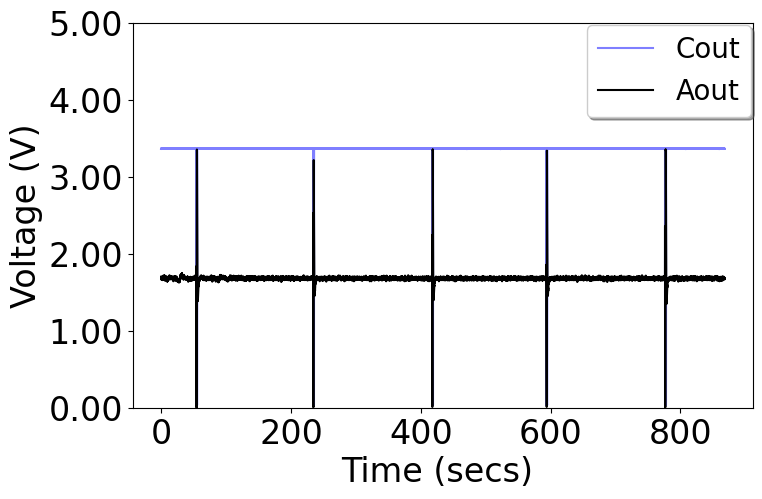
\includegraphics[width=\textwidth]{figures/gradual_degradation_dust/Stage0.png}
		\caption{Clean Sensor : Working}
		\label{fig:pir_sensor_classIII_fault_good}
	\end{subfigure}
	\hspace{1ex}
	\begin{subfigure}[t]{0.23\textwidth}
		\centering
		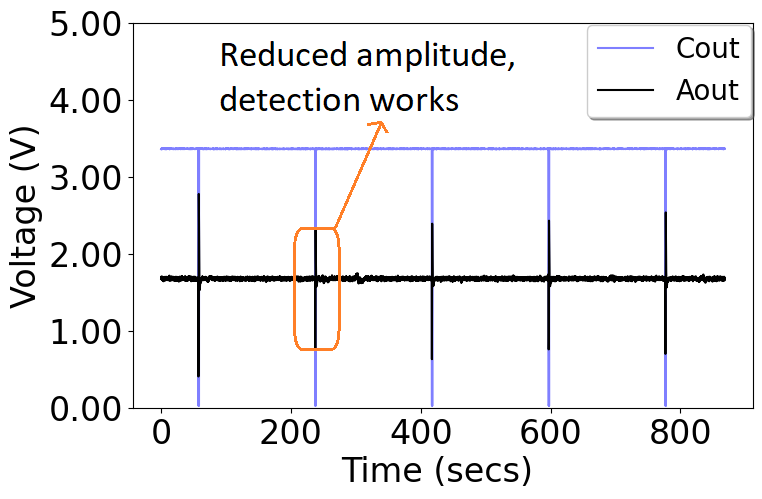
\includegraphics[width=\textwidth]{figures/gradual_degradation_dust/Stage1.png}
		\caption{Degraded Sensor : Still Working}
		\label{fig:pir_sensor_classIII_fault_bad1}
	\end{subfigure}	
	\hspace{1ex}
	\begin{subfigure}[t]{0.23\textwidth}
		\centering
		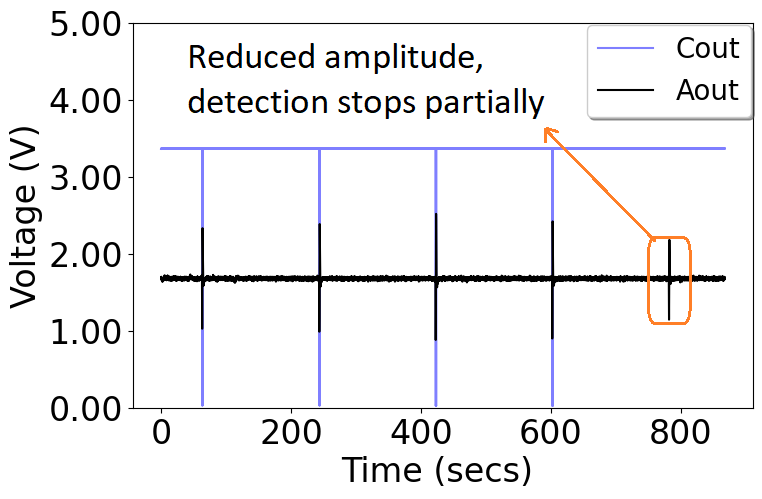
\includegraphics[width=\textwidth]{figures/gradual_degradation_dust/Stage2.png}
		\caption{Degraded Sensor : 1/5 miss}
		\label{fig:pir_sensor_classIII_fault_bad2}
	\end{subfigure}		
	\hspace{1ex}
	\begin{subfigure}[t]{0.23\textwidth}
		\centering
		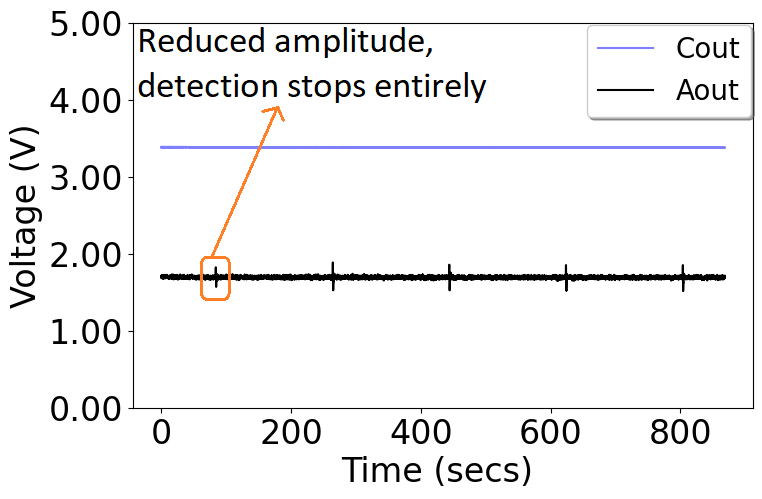
\includegraphics[width=\textwidth]{figures/gradual_degradation_dust/Stage3.png}
		\caption{Failed Sensor : 5/5 miss}
		\label{fig:pir_sensor_classIII_fault_bad3}
	\end{subfigure}	
	\caption{Dust gradually building up in different degrees causing Class III faults -- \ca is a clean sensor and dust gradually builds up \cb -- \cd at which stops detecting obstacles.}
	\label{fig:pir_sensor_classIII_fault_gradual}
\end{figure*}

%\subsubsection{Gradual Degradation in Class III faults} 
To study the effect of gradual failures occurring in Class III, we divided a spatula of chalk-dust (approximately one-fourth of a teaspoon) and measured the effect of dust on response of the sensor. At every stage of study, we incrementally added dust and measured performance by plotting the two output signals \cout and \aout in the presence of an obstacle. The experiment is summarized in {\bfseries Fig.~\ref{fig:pir_sensor_classIII_fault_gradual}}. With increasing amount of dust being deposited, we see that the final discrete output misses the obstacle on occasion while detecting it sometimes. As a result, information about the dust deposition is lost at times from the final discrete output, \cout. \textit{Note that however, the intermediate analog output, \aout is able to capture information regarding the deposition of dust and by showing the degradation of sensing performance via its reduced amplitude.} Consequently, the obstacle detection process works till a reduced amplitude of \aout ({\bfseries Fig.~\ref{fig:pir_sensor_classIII_fault_bad1}}), below which the sensor begins missing some obstacle instances. This process aggravates as more dust is accumulated on the sensor until a stage when there is a complete failure ({\bfseries Fig.~\ref{fig:pir_sensor_classIII_fault_bad3}}).

\noindent \textbf{Summary:} The key observation here is that capturing the physics of sensing via \aout helps glean valuable insights into even partial failures, which is completely absent in the \cout signal.


\subsection{Analysis of \aout during known quiet times} \label{subsec:aout_quiet_times} We draw some intuition on the behavior of \aout during known times of no occupancy, \eg post business hours in case of office buildings. The intuition stems from the arrangement of pyroelectric elements and its interplay with the lens subsystem. In a working sensor, we observe that due to the precise geometric arrangement of lens and pyroelectric elements, when there is no obstacle, the thermal radiation from the environment falls equally on the two pyroelectric elements, causing it to cancel out and leave very little noise at the output of pyroelectric subsystem. However, when the lens is covered by a foreign substance (\ie Class III fault), some of the thermal radiation is absorbed by the substance, before falling onto the pyroelectric elements. This results in a much lower noise at the output of pyroelectric subsystem. Alternately, if the lens is dislodged (\ie Class I fault), the two pyroelectric elements are not perfectly matched in differential configuration, which leads to higher noise at output of the pyroelectric subsystem. We observe this noise by measuring the \textit{noise floor} in the variance of \aout signal, during times of no obstacle.

Thus, we note that variance of \aout during a period with no occupancy can be used to get hints on Class I (lens dislodged) and Class III faults (lens covered). In particular, compared to a working sensor where the lens is mounted correctly, we expect a drop in variance when the lens is covered and a rise in variance when the lens is dislodged. In other words, $\sigma$(\aout)$|_{Class\ III}$ $\leq$ $\sigma$(\aout)$|_{Working}$ $\leq$ $\sigma$(\aout)$|_{Class\ I}$, where $\sigma$(\aout)$|_{X}$ denotes the variance of \aout under scenario X. We can use this idea to develop a preliminary fault detection algorithm that can be used to screen for lens faults (Class I and III). This requires computing two variance-based thresholds ($T_L$, $T_H$) to deduce status of the lens.

However, we note that using the variance of \aout is not viable in all practical conditions. In particular, using this method works only during \textit{known quiet} times \ie in the known absence of occupancy which can be a \textit{disadvantage} for some deployments. As a result, this approach is suited for preliminary sensor health checks outside office or regular business hours of operation such as weekends. %Therefore, we need to perform additional characterization of the \aout output signal to reason about the failures in a more systematic manner.

% ashish
\begin{wrapfigure}{L}{10cm}%[ht]
	\centering
	\begin{subfigure}[t]{0.3\textwidth}
		\centering
		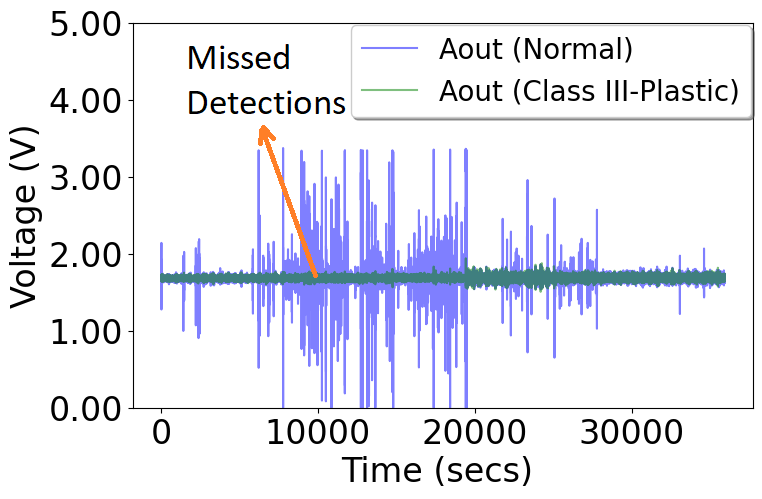
\includegraphics[width=\textwidth]{figures/2-PIR-Fault/normal-classIII/Aout_normal_vs_plastic.png}
		\caption{Plastic}
		\label{fig:pir_sensor_classIII_fault_plastic_tape}
	\end{subfigure}
	\begin{subfigure}[t]{0.3\textwidth}
		\centering
		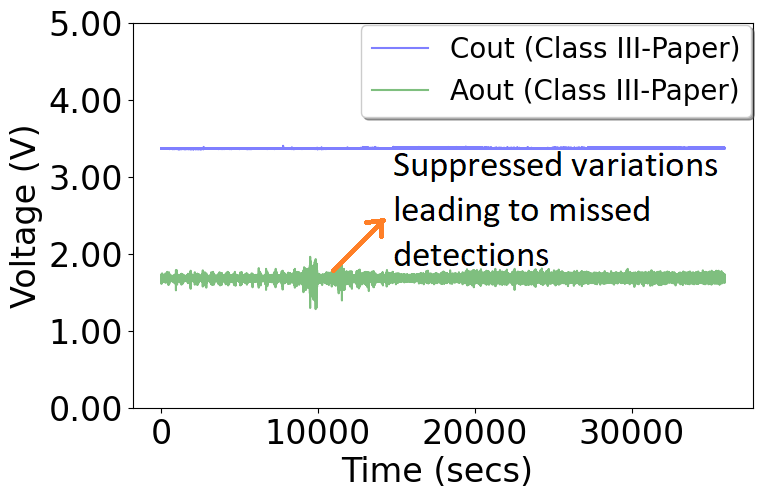
\includegraphics[width=\textwidth]{figures/2-PIR-Fault/normal-classIII/Cout_Aout_Paper.png}
		\caption{Paper}
		\label{fig:pir_sensor_classIII_fault_paper}
	\end{subfigure}	
	\caption{Effect of different foreign particles producing Class III faults of different degree -- the figures show that when the lens is obstructed with foreign particles like plastic tape and paper, it could result in complete failure.}
	\label{fig:pir_sensor_different_foreign_particles}
\end{wrapfigure}

\subsection{Analysis of different types of foreign particles} \label{subsec:foreign_additional}Different materials have distinct thermal characteristics and thus affect the \aout response differently in case of Class III faults. Stated alternately, the amplitude shaping of \aout varies depends on the material and its quantity. There are 3 kinds of foreign particles we study in our setup -- \ca paper, \cb plastic tape and \cc dust. We saw in {\bfseries Fig.~\ref{fig:pir_sensor_controlled_c}} how deposition of dust can compromise with the \aout responses. {\bfseries Fig.~\ref{fig:pir_sensor_different_foreign_particles}} shows Class III fault scenarios repeated with plastic tape and paper. In each of these runs, a normal sensor (represented in the blue curve in {\bfseries Fig.~\ref{fig:pir_sensor_classIII_fault_plastic_tape}}) detects obstacles as demonstrated by the \aout variation, whereas foreign particles such as paper and plastic tape can lead to a \textit{complete failure} of the PIR sensor.
%The response of the sensor can vary depending on the extent of obstruction as well as nature of the material obstructing the lens. In our experiments, we see that foreign particles such as paper and plastic tape can lead to a \textit{complete failure} of the PIR sensor.

%%%%%%%%%%
%%% MOVED THIS TO APPENDIX
%%%%%%%%%%%%

\begin{comment}
\textbf{Note:} The variance of \aout during a period with no obstacle can be used to get hints on Class I faults (lens dislodged) and Class III faults (lens covered). In particular, compared to a working sensor where the lens is mounted correctly, we observe a drop in variance when the lens is covered and a rise in variance when the lens has fallen. In other words, $\sigma$(\aout)$|_{Class\ III}$ $\leq$ $\sigma$(\aout)$|_{Working}$ $\leq$ $\sigma$(\aout)$|_{Class\ I}$, where $\sigma$(\aout)$|_{X}$ denotes the variance of \aout under scenario X. We extend this to develop a preliminary fault detection algorithm that can be used to detect Class I and Class III faults. This requires the computation of two variance-based thresholds ($T_L$, $T_H$) to deduce the status of the lens. 

However, we note that using the variance of \aout is not viable in all practical conditions. In particular, this method works only during \textit{quiet} times \ie in the absence of an obstacle which is a \textit{disadvantage}. As a result, this approach is suited for outside office or regular business hours of operation such as weekends. Therefore, we need to perform additional characterization of the \aout output signal to reason about the failures.
\end{comment}
%%%%%%%%%%
%%% END MOVED THIS TO APPENDIX
%%%%%%%%%%%%

% \noindent \textbf{Summary:} The analog output (\aout) allows us to `peek under the hood' into the physics of a PIR sensor which is invaluable in case of failures.

\begin{comment}
\subsection{Time Domain Characterization} We ask ourselves the question -- `What can we learn from only the time domain representation of \aout ?' Recall from {\bfseries Fig.~\ref{fig:pir_sensor_controlled_a}}, that we observed the variance of \aout during a period of no obstacle is a key indicator of lens fault\ie \ca lens being covered (say due to a foreign particle) or \cb lens falls off completely (say due to imperfect bonding). We compare this with the case where lens cap is mounted correctly. 

% This happens because the lens serves to focus the incident infrared radiation into the  optical arrangement of the pair of pyroelectric elements connected in a serially opposite manner. Therefore, when there is no obstacle present, both the pyroelectric elements are exposed to the same magnitude of incident radiation, and due to their opposing connection, the output is nullified. The absence of the fresnel lens leads to the induced voltages not cancelling exactly due to dispersion effects. 

We deployed three sensors over lunchtime in an office cafeteria : \ci a working sensor, \cii a sensor with lens covered with tape, and \ciii a sensor with lens fallen (removed). This time-domain behavior of \aout in these cases is summarized in {\bfseries Fig.~\ref{fig:variance_cap_cases}}.  We observe a drop in variance when the lens is covered and a rise in variance if the lens falls off. In other words, $\sigma$(\aout) $|_{Covered}$ $\leq$ $\sigma$(\aout) $|_{Working}$ $\leq$ $\sigma$(\aout) $|_{No\ Lens}$, where $\sigma$(\aout) denotes the variance of \aout.

Extending this we develop a threshold-based fault detection algorithm (Algorithm~\ref{alg:fault_detection}) that can be used to detect simple faults in lens. This requires the computation of variance-based thresholds ($T_L$, $T_H$) to find the status of the lens.%if the lens is covered, is fallen off or if the lens is working as intended.

Despite the theoretical correctness of this time-domain approach, we note that using variance of \aout is not viable in all practical conditions. In particular, it has the \textit{disadvantage} that it works only during \textit{quiet} times \ie requiring the absence of an obstacle. Thus, this approach is suited for outside office or regular business hours of operation such as weekends.

Consequently, we look for other approaches of characterizing the \aout waveform.

% We note that using variance of \aout to characterize lens cap related faults relies on the absence of an obstacle and can detect only extreme failures. Thus, this approach is suited for outside office or regular business hours of operation such as weekends.

\end{comment}

%%%%%%%%%%
%%% FREQUENCY DOMAIN REPRESENTATIONS
%%%%%%%%%%%%

\begin{figure}%[htbp]
	\centering
	%\vspace*{-1.5\baselineskip}
	\begin{subfigure}[t]{0.33\textwidth}
		\centering
		%\includegraphics[width=\linewidth]{figures/2-PIR-Fault/normal-classI/obstacle_classIfault_vs_normal-tightfit.png}
		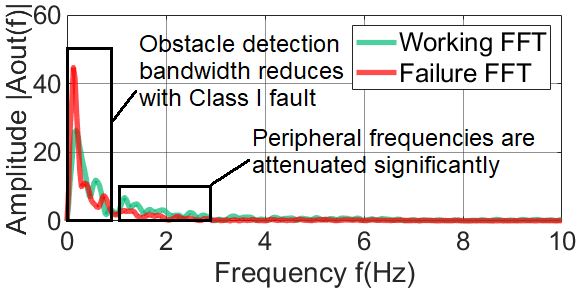
\includegraphics[width=\textwidth]{figures/2-PIR-Fault/normal-classI/class1_fft_coloradj_small_edited_camera_ready.png}
		\caption{Class I fault}
		\label{fig:classI_fault_freq}
	\end{subfigure}
	\begin{subfigure}[t]{0.33\textwidth}
		\centering
		% \includegraphics[width=\linewidth]{figures/2-PIR-Fault/normal-classII-deformed/obstacle_classIIdeformedfault_vs_normal-faultshows-tightfit.png}
		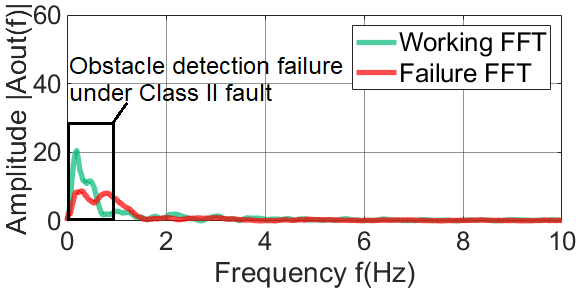
\includegraphics[width=\textwidth]{figures/2-PIR-Fault/normal-classII-deformed/class2_fft_coloradj_small_edited_camera_ready.png}
		\caption{Class II fault}
		\label{fig:classII_fault_freq}
	\end{subfigure}
	\begin{subfigure}[t]{0.325\textwidth}
		\centering
		%\includegraphics[width=\linewidth]{figures/2-PIR-Fault/normal-classIII/obstacle_classIIIdeformedfault_vs_normal-faultshows_510000to525000-tightfit.png}
		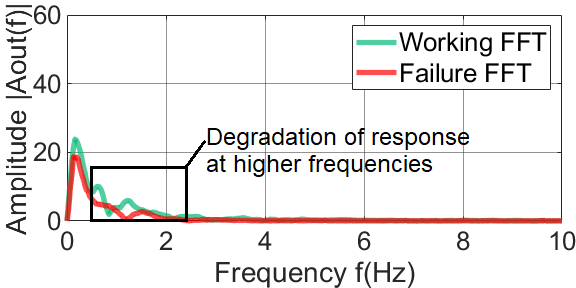
\includegraphics[width=\textwidth]{figures/2-PIR-Fault/normal-classIII/class3_fft_coloradj_small_edited_camera_ready.png}
		\caption{Class III fault}
		\label{fig:classIII_fault_freq}
	\end{subfigure}\\
	\begin{subfigure}[t]{0.33\linewidth}
		\centering
		%\includegraphics[width=\linewidth]{figures/2-PIR-Fault/normal-classIV/obstacle_classIVdeformedfault_vs_normal-faultshows_210000to225000-tightfit.png}
		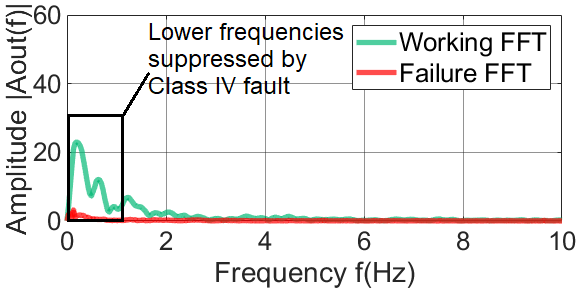
\includegraphics[width=\linewidth]{figures/2-PIR-Fault/normal-classIV/class4_fft_coloradj_small_edited_camera_ready.png}
		\caption{Class IV fault}
		\label{fig:classIV_fault_freq}
	\end{subfigure}
	\begin{subfigure}[t]{0.33\linewidth}
		\centering
		%\includegraphics[width=\linewidth]{figures/2-PIR-Fault/normal-classV/obstacle_classVdeformedfault_vs_normal-faultshows_390000to405000-tightfit.png}
		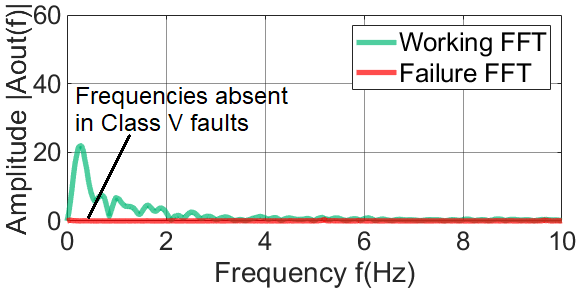
\includegraphics[width=\linewidth]{figures/2-PIR-Fault/normal-classV/class5_fft_coloradj_small_edited_camera_ready.png}
		\caption{Class V fault}
		\label{fig:classV_fault_freq}
	\end{subfigure}
	\begin{subfigure}[t]{0.325\linewidth}
		\centering
		%\includegraphics[width=\linewidth]{figures/2-PIR-Fault/normal-normal/obstacle_normal_vs_normal-tightfit-2.png}
		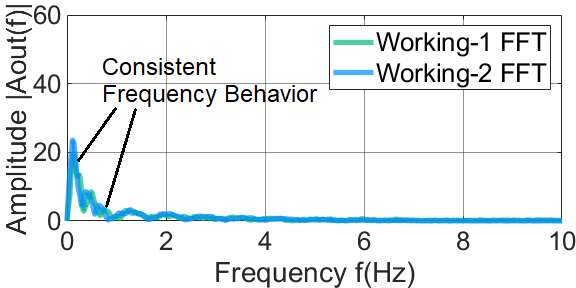
\includegraphics[width=\linewidth]{figures/2-PIR-Fault/normal-normal/normal_normal_fft_coloradj_small_edited_camera_ready.png}
		\caption{\textbf{Comparing} \aout of two working sensors}
		\label{fig:normal_normal_freq}
	\end{subfigure}
	\caption{\footnotesize{Frequency Domain Representations} of \aout under different faults in a PIR sensor. Only frequencies upto 10 Hz are shown as most PIR sensors detect human motion within 10 Hz.}
	\label{fig:classI-V_fault_freq}	
\end{figure}
%\begin{figure}
%	\centering
%	%\includegraphics[scale=0.49]{figures/2-PIR-Fault/normal-classIV/obstacle_normal_run4.png}
%	%\includegraphics[scale=0.49]{figures/2-PIR-Fault/normal-classIV/obstacle_classIVfault.png}
%	\includegraphics[width=0.99\columnwidth]{figures/2-PIR-Fault/normal-classV/obstacle_classVdeformedfault_vs_normal-faultshows_390000to405000-tightfit.png}
%	\caption{\textsc{Frequency Domain Representation} of \aout under an electronic subsystem fault.}
%	\label{fig:classV_fault_freq}
%\end{figure}
%%%%%%%%%%
%%% END FREQUENCY DOMAIN REPRESENTATIONS
%%%%%%%%%%%%
\subsection{Frequency Domain Characterization} \label{subsec:freq_char} %To further characterize the \aout waveform, 
We have showed \aout signal has hints about various failure scenarios. %This indicated that we need to perform careful characterization of the \aout output signal to reason about the failures in a more systematic manner. 
To get additional insights, we transform the time domain \aout signal into frequency domain using the Fast Fourier transform (FFT) to derive robust features. FFT offers high resolution in the frequency domain and deconstructs the frequencies and harmonics present in a signal. Frequency domain representations have been used to characterize human activities using smartphone sensors and perform vibration screening for faults both in aircraft and railway lines~\cite{anguita2013public, HanlyWhy}. 

We plot the FFT representations of \aout corresponding to different faults in {\bfseries Figs.~\ref{fig:classI_fault_freq}--~\ref{fig:classV_fault_freq}} as compared to a working sensor, all under the presence of an obstacle. The y-axis plots magnitude of FFT coefficients and the x-axis plots frequencies in the human range of motion (0 -- 10 Hz). In case of a working sensor, we observe 2 big peaks and additional peripheral frequencies up to 4 Hz. We now study how the frequency spectrum varies depending on the type of faults.

%We also note the FFT of the \aout for a working sensor under an obstacle. Note that the frequency distribution is between 0 -- 10 Hz, which is the range triggered by human motion. We observe a 2 big peaks and peripheral frequencies upto 4 Hz. 

\textbf{Class I faults}  %Recall from \S\ref{subsec:taxonomy} that in a Class I fault, the lens cap gets dislodged, either completely or partially, which causes the thermal radiation to fall imperfectly on the optical lens. We earlier saw in Fig.~\ref{fig:pir_sensor_controlled_b}, the impact of a Class I fault on \aout and \cout. Intuitively, we expect that the Class I faults lead to two phenomena -- \ca reduced capture and focus of the thermal radiation, and \cb presence of additional frequencies due to leakage thermal radiation. In addition, when an obstacle is not present, a dislodged lens cap leads to imperfect balance of the differential pyroelectric element and this results in some low-value at the output. 
We observe in \textbf{Fig.~\ref{fig:classI_fault_freq}} that a dislodged lens cap (either partial or complete) leads to reduced information capture (lower bandwidth) and as a result, the sensitivity in the periphery of the sensors reduces. Note that there is just a single prominent peak in the faulty sensor (at a slightly lower frequency when compared to the normal sensor) that corresponds to the obstacle being perfectly aligned with the center of sensor as it passes. The magnitude reduces sharply as it moves away from the center of the sensor. %This is expected as the lens cap is crucial for focusing the thermal radiation.

\textbf{Class II faults} %caused due to structural damage to the lens itself (~\eg puncture or deformation), can manifest itself in reduced detection performance as some of the detection region become \textit{blind spots} for the sensor. As a result, there are additional neighbouring frequencies triggered along with the primary frequency of the obstacle as seen in  
\textbf{Fig.~\ref{fig:classII_fault_freq}} plots the FFT for a sensor with deformed lens cap. 
%We damage the lens by deforming the lens cap leading to compromise of its curvature that is responsible for focusing thermal radiation. 
%In this scenario, the lens cap damage 
We note that Class II faults lead to significantly suppressed primary peaks (approx. 10 db). In addition, the peripheral frequencies are attenuated as observed in Class I. These faults can manifest itself in reduced sensor performance as some of the detection region become \textit{blind spots} for the sensor.

%-- this also aligns with the reduced amplitude of the \aout signal in Figure~\ref{fig:pir_sensor_controlled_b}.

\textbf{Class III faults} due to accumulation of foreign particles in the lens, lead to reduced sharpness of frequencies.
%The overall flattening of the frequency response continues with increased deposition of foreign materials until it reaches a stage where the primary frequency spike is no longer discernible. 
%\textbf{Summary (Figure~\ref{fig:classIII_fault_freq})} We deposit foreign material (dust) on the lens cap leading to reduced thermal radiation reaching the pyroelectric element as some of it is absorbed by the foreign substance. Naturally, different amounts and types of foreign substance lead to different detection performance. 
We observe in \textbf{Fig.~\ref{fig:classIII_fault_freq}} that the degradation starts with damping of the higher frequencies. As the amount of dust increases, we observe the frequencies getting increasingly damped until the object detection starts failing.


\textbf{Class IV faults}
%due to damage of the optical filter in front of the pyroelectric element, can also result in poor detection performance and attenuation of frequencies in the output. The damage in this case can be caused by humidity or impurities. 
%We study the effect of contamination of the optical filter with humidity by spraying oil on the optical filter.
We observe in \textbf{Fig.~\ref{fig:classIV_fault_freq}} that the frequencies present in the output are heavily suppressed resulting in missed obstacle detection. This is expected since the optical filter plays a major role in filtering out the non-human range frequencies from the thermal radiation and only passing through the frequencies corresponding to the human range. The presence of oil condensation or heat sinks causes absorption of the thermal radiation resulting in insufficient heat to cause pyroelectric effect. 

\textbf{Class V faults} such as open and short circuits are %caused to electronic faults such as short circuits on the sensor boards. These types of faults are 
easy to detect due to the absence of any prominent frequencies. Consequently, \aout is \textit{stuck at} a value leading to only dc frequencies being present in the output. This result is observed in {\bfseries Fig.~\ref{fig:classV_fault_freq}}, where the \cout and \aout pins are shorted on the board. 

\noindent \textbf{Summary:} %The FFT representation of \aout allows us to capture the harmonics of a PIR sensor. 
Frequencies present in FFT representations of \aout provide hints regarding status (\ie working/failed) of PIR sensors.

%We now have frequency distributions (in terms of FFT coefficients) of \aout for each class of failed sensor and working sensor.
% \subsection{Problem Statement Revisited}
% The problem of fault detection and isolation is now reduced to that of matching the characteristics (\ie physics) of collected \aout waveforms with each of the failure scenarios. This is a compute and data-intensive problem due to the complexity of features \eg variance, frequency spectrum and the corresponding amplitudes. As a result, we use insights from machine learning \viz Benjamini-Hochberg (B-H) feature selection and Shapley values in conjunction with Random Forest classifiers to : \ca isolate and distinguish between working and faulty sensors (\ie fault detection) and  \cb rootcause the fault present by assigning it to the correct class of failure (\ie fault diagnosis).

%In our case, we use 1024-point FFT coefficients (resulting in 512 FFT coefficients) generated every 50 ms (details described later). 

%%%%%%%%%%
%%% CDF REPRESENTATIONS
%%%%%%%%%%%%


%\begin{figure*}[h]
%%\centering
%	\subfloat[Class I fault \label{fig:classI_fault_cdf}]{%
%		\includegraphics[scale=0.49]{figures/2-PIR-Fault/normal-classI/CDF_Comparison_150000_to_165000.png}}
%	\subfloat[Class II fault \label{fig:classII_fault_cdf}]{%
%		\includegraphics[scale=0.49]{figures/2-PIR-Fault/normal-classII-deformed/CDF_Comparison_210000_to_225000.png}}\\
%	\subfloat[Class III fault \label{fig:classIII_fault_cdf}]{%
%		\includegraphics[scale=0.49]{figures/2-PIR-Fault/normal-classIII/CDF_Comparison_90000_to_105000.png}}
%	\subfloat[Class IV fault \label{fig:classIV_fault_cdf}]{%
%		\includegraphics[scale=0.49]{figures/2-PIR-Fault/normal-classIV/CDF_Comparison_210000_to_225000.png}}
%    \caption{\textsc{CDF Representations} of \aout under lens and pyroelectric subsystem faults in a PIR sensor.}
%\label{fig:classI-IV_fault_cdf}
%\end{figure*}
%
%\begin{figure}
%\centering
%%\includegraphics[scale=0.49]{figures/2-PIR-Fault/normal-classIV/obstacle_normal_run4.png}
%%\includegraphics[scale=0.49]{figures/2-PIR-Fault/normal-classIV/obstacle_classIVfault.png}
%\includegraphics[scale=0.49]{figures/2-PIR-Fault/normal-classV/CDF_Comparison_210000_to_225000.png}
%\caption{\textsc{CDF Representation} of \aout under an electronic subsystem fault.}
%\label{fig:classV_fault_cdf}
%\end{figure}
%

%\begin{figure}
%\centering
%%\includegraphics[width=\columnwidth]{figures/2-PIR-Fault/normal-normal/Aout_CDF_comparison_both_working.png}
%\includegraphics[width=\columnwidth]{figures/2-PIR-Fault/normal-normal/Aout_Freq_comparison_both_working.png}%
%\caption{\textsc{Comparison between} \aout of two working sensors show consistency in their frequency distributions}
%\label{fig:normal_normal_freq}
%\end{figure}

%%%%%%%%%%
%%% END CDF REPRESENTATIONS
%%%%%%%%%%%%

